\section{Results}
\label{sec:results}

These are the kinds of graphs we are going to make from the simulation. These 
does not represent what we will actually have in the report, since there is 
still calibration etc. to be done. We haven't started doing analysis of them 
yet either. They are just put here to give an idea of what it is we will be 
getting from all of this.

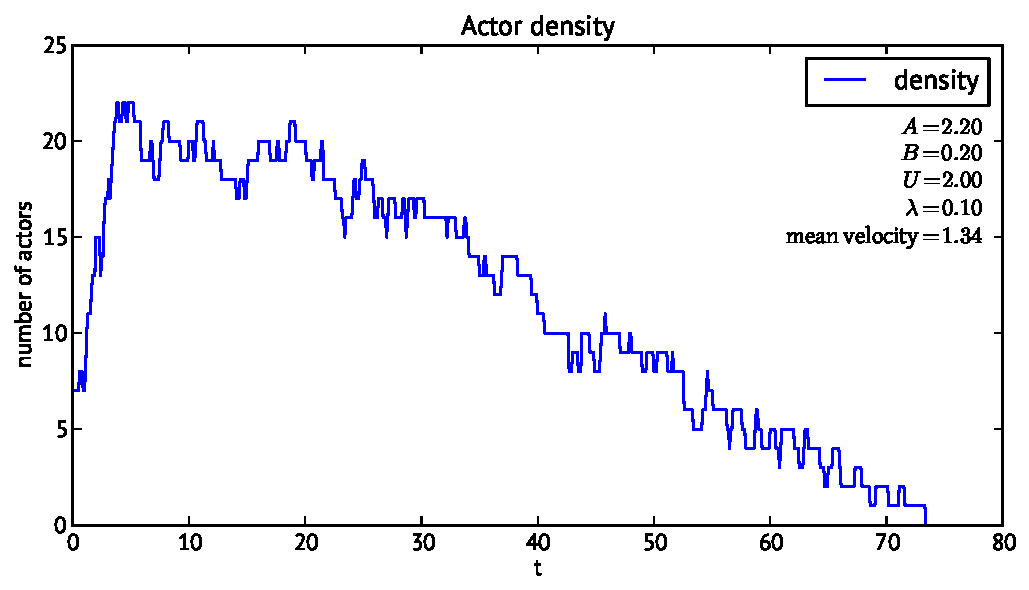
\includegraphics[width=0.5\textwidth]{Figures/plots/square_room-density.pdf}
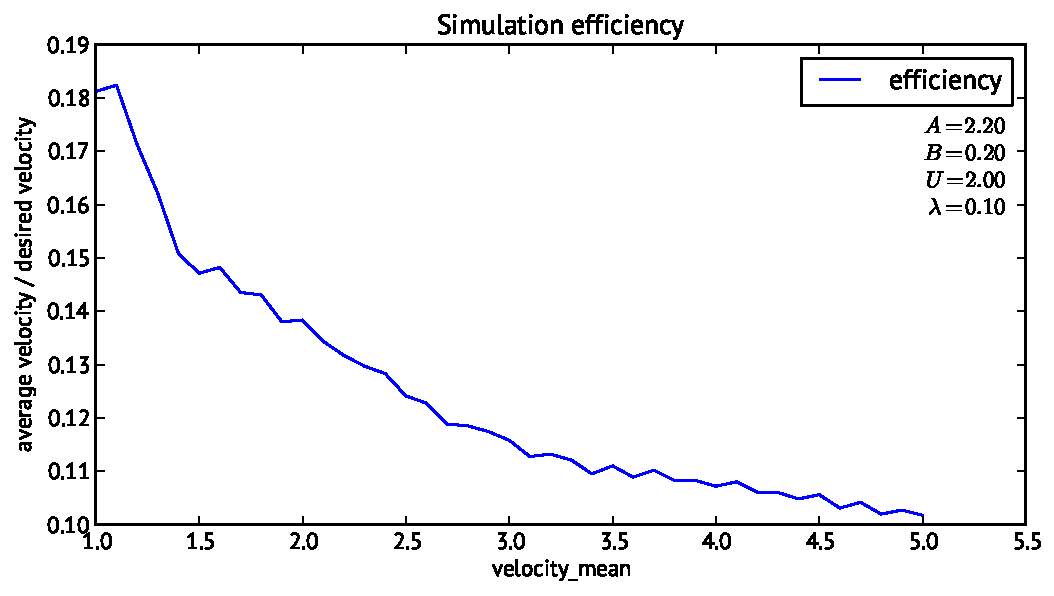
\includegraphics[width=0.5\textwidth]{Figures/plots/square_room-efficiency-aggr-velocity_mean.pdf}
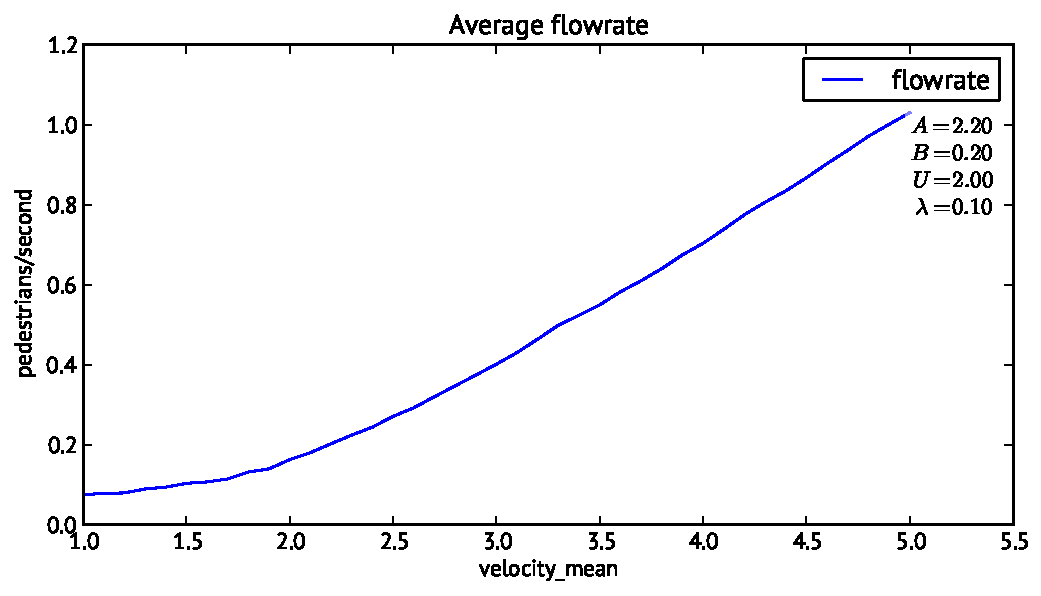
\includegraphics[width=0.5\textwidth]{Figures/plots/square_room-flowrate-aggr-velocity_mean.pdf}
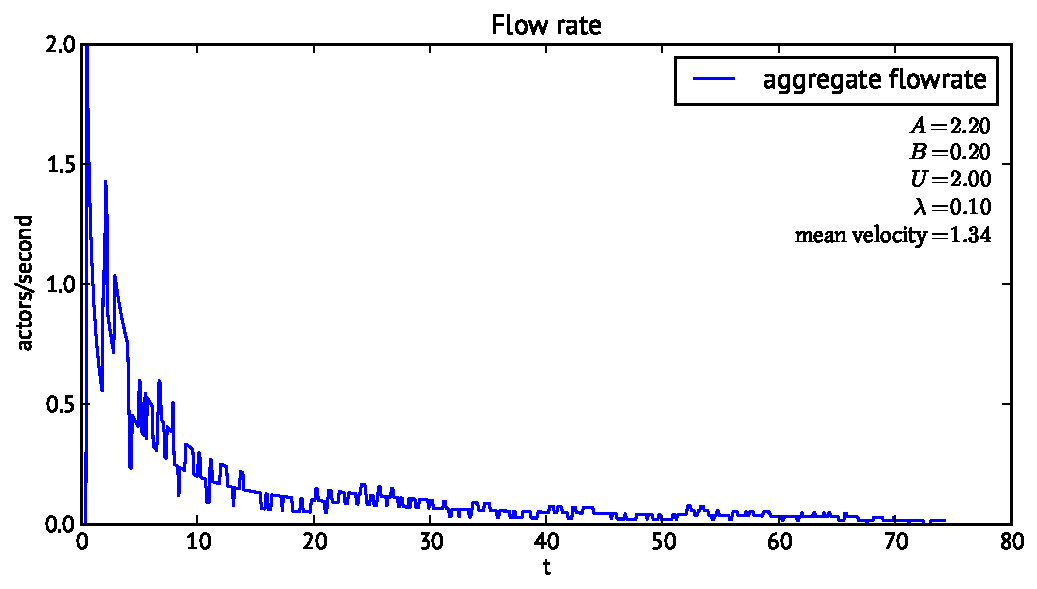
\includegraphics[width=0.5\textwidth]{Figures/plots/square_room-flowrate.pdf}
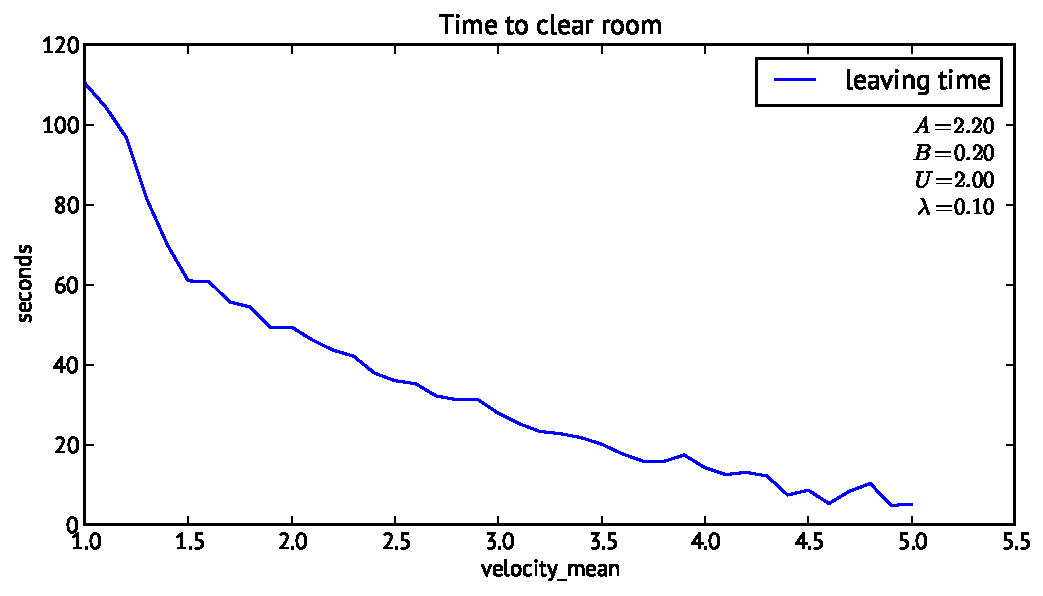
\includegraphics[width=0.5\textwidth]{Figures/plots/square_room-leaving_time-aggr-velocity_mean.pdf}
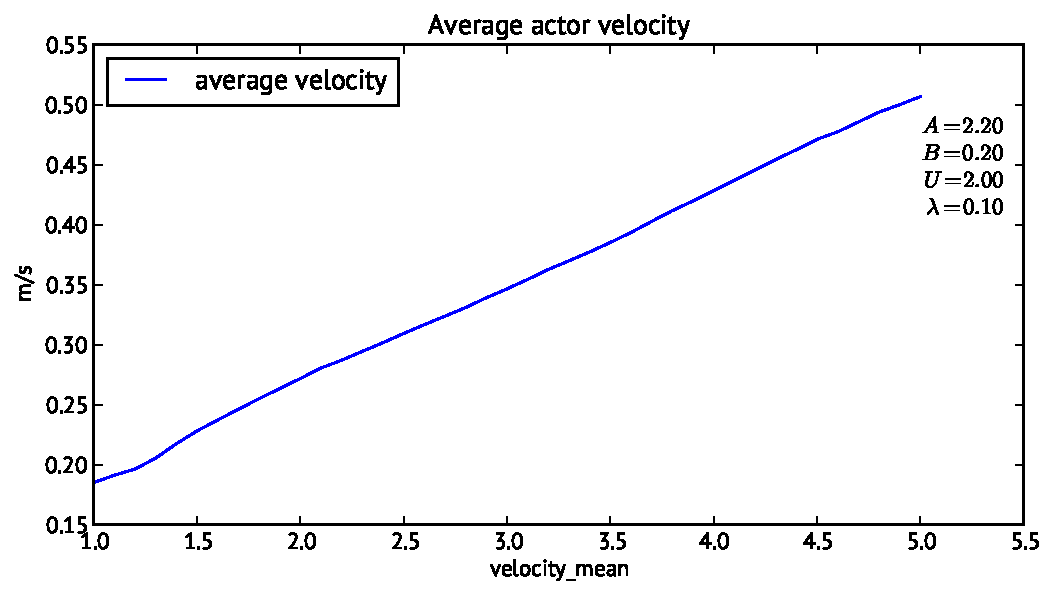
\includegraphics[width=0.5\textwidth]{Figures/plots/square_room-velocity-aggr-velocity_mean.pdf}
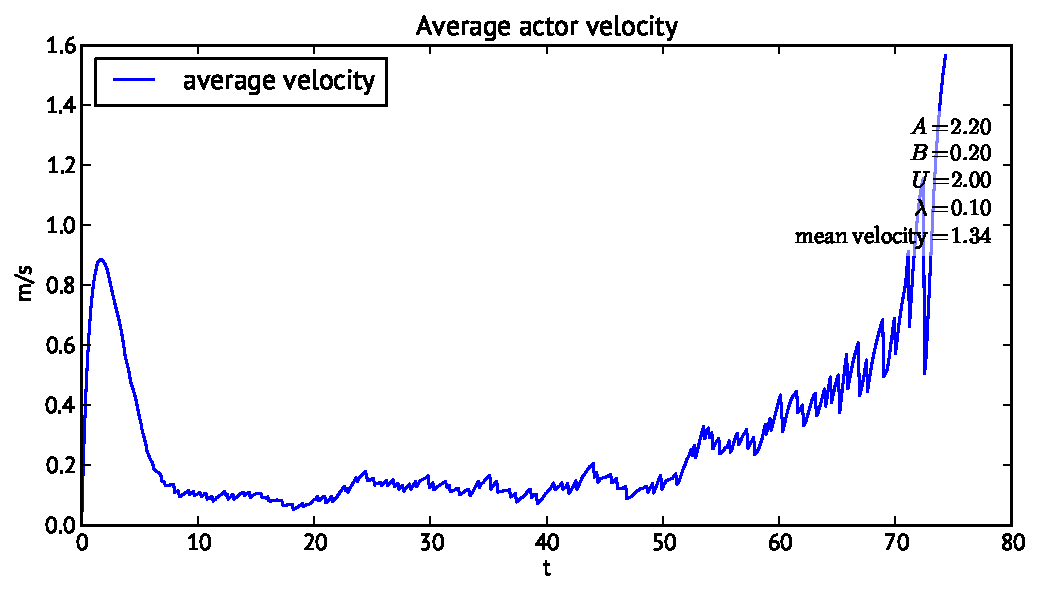
\includegraphics[width=0.5\textwidth]{Figures/plots/square_room-velocity.pdf}

\subsection{Lane Formation}
Especially in counterflow situation, pedestrians form lanes of walking directions, which is thought as a result of the non-linear body interaction force.

\subsection{Oscillatory Flows at Bottlenecks}
In bidirectional flow situations, each direction takes turns to pass the bottleneck.

\subsection{Freezing by Heating Effect}
This phenomenon is characterized by a blockage that follows an increasing density. The precondition for this effect is the driving force from desired velocity and actual velocity, while the tangential term from the interaction force is not needed.

\subsection{Faster-Is-Slower Effect}
It has been observed in evacuations situations that some process takes more time if it is performed at high speed. In our simulation, in order to see this effect, we need to have the body repulsion and friction force.